\documentclass[11pt,a4paper]{scrartcl}
\usepackage{flupstyleutf}
\usepackage{ae}
\usepackage[bitstream-charter]{mathdesign}
\usepackage[parfill]{parskip}


\defbibheading{partitions}{\subsection*{Partitions}}
\defbibheading{theorie}{\subsection*{Ouvrages musicaux}}

%\DeclareGraphicsExtensions{.pdf, .jpg, .tif}
\title{LA VALLÉE D'OBERMANN\\ de Franz Liszt}
\author{Philippe Massart}
\pagestyle{fancy}
\lhead{La Vallée d'Obermann}        \chead{}        \rhead{}

\begin{document}
\titlepage
\date {juin 1995}
%\maketitle
\begin{center}
{\large \textbf{LA VALLÉE D'OBERMANN}} \\de Franz Liszt \vspace{2cm}
\\Philippe Massart\vspace{16cm}
\\juin 1995
\\Conservatoire Royal de Bruxelles
\\Cours d'histoire de la musique --- Classe de M. STOCKHEM
\end{center}
\newpage
\newpage
\section{Biographie succincte de Franz Liszt}

Franz Liszt naît à Raiding (Hongrie) en 1811, Son père, employé à la cour d'Esterhazy, était un musicien amateur.
À l'âge de neuf ans, l'extraordinaire talent pianistique du jeune garçon lui vaut une bourse qui lui permet d'aller étudier à Vienne chez Czerny et Salieri;
il y rencontrera également Schubert et Beethoven. En 1823, il s'installe à Paris.
C'est au cours des années qui suivent que se dégagent les aspects essentiels de sa nature:
une attirance mystique vers la religion, un besoin très profond d'attachements féminins et une volonté déterminée
d'élargir la technique pianistique (influencé en cela par la virtuosité de Paganini).

Le piano sera donc son moyen d'expression privilégié. Il se lie avec la comtesse Marie d'Agoult qu'il emmène en
Suisse et en Italie; les deux premiers cahiers des \emph{Années de Pèlerinage} datent de cette époque.
De 1840 à 1847, il parcourt l'Europe, de récitals en concerts. Mais il se lasse de cette vie mondaine et,
en septembre 1847, renonce à sa carrière de virtuose et se consacre à l'enseignement.

En 1848, Liszt s'installe à Weimar, C'est de cette période que date la majeure partie de son \oe{}uvre symphonique
(les poèmes symphoniques, deux symphonies, deux concertos pour piano)
et pianistique (\emph{Sonate en si mineur}, \emph{Rhapsodies hongroises}, \emph{Etudes d'exécution transcendante} etc. )
En tant que chef d'orchestre, Liszt se fait le champion d'autres compositeurs: Beethoven, Schubert
(encore peu connu à l'époque), Berlioz et surtout Wagner.

En 1861, il s'installe à Rome, espérant jouer un rôle important dans la vie musicale de l'Eglise; de cette époque datent
ses deux oratorios (\emph{Sainte Elisabeth} et \emph{Christus}), ainsi que des \oe{}uvres d'inspiration religieuse pour piano et pour orgue,
À cette époque, sa fille Cosima est l'amante de Wagner, et leurs relations se détériorent. En 1865, Liszt rejoint les ordres
mineurs et mène une vie quasi monastique, Les dernières années de sa vie seront marquées par sa réconciliation avec
Cosima et Richard Wagner, la mort de ce dernier (en 1883) et quelques \oe{}uvres qui annoncent l'évolution
stylistique des années suivantes.

\section{Les Années de Pèlerinage}

Les \emph{Années de Pèlerinage} sont composées de trois livres. Rédigé à partir de 1836, mais reprenant en partie des
éléments d'un recueil intitulé d'abord \emph{Album d'un voyageur}, le premier livre (\emph{Suisse} ou \emph{Première Année})\footcite{liszt:pelerinage1} ne fut
publié qu'en 1855: ses neuf pièces évoquaient le séjour et les excursions entreprises à travers la Suisse quelque vingt ans
plus tôt en compagnie de Marie d'Agoult. Le rôle de cette dernière se révèlera très important dans ce recueil: c'est grâce
à elle que Liszt découvrira la littérature française, et entre autres, Etienne de Senancour.

Composé entre 1837 en 1849, publié en 1858, le deuxième livre --- \emph{Italie} ou \emph{Deuxième Année}\footcite{liszt:pelerinage2} --- fut consacré lui aussi aux
souvenirs d'un voyage avec Marie d'Agoult. Toutefois ses sept pièces reflétaient une évolution dans la pensée musicale
de Liszt: les centres d'intérêt s'étaient en effet déplacés vers la littérature (Dante, Pétrarque) et vers la peinture et la
sculpture (Raphaël, Michel-Ange), établissant des correspondances entre les arts et préfigurant, d'une certaine manière,
la synthèse bientôt tentée par Richard Wagner dans ses opéras.
À ce deuxième cahier furent annexées trois pièces mineures, publiées en 1859, regroupées sous le titre
\emph{Venezia e Napoli}.

Beaucoup plus tardif que les précédents, le troisième livre enfin --- \emph{Troisième Année}\footcite{liszt:pelerinage3} --- comprend sept pièces écrites entre
1867 et 1877: leur publication n'intervint qu'en 1883, trois ans avant la mort du compositeur. Nouvel et dernier aspect
du génie musical de Liszt, qui avait reçu les ordres mineurs en 1865.

L'idée des \emph{Années de Pèlerinage} n'est pas la description littérale d'un paysage ou d'un monument, mais bien l'évocation
d'impressions, de sentiments stimulés par tel paysage ou monument. Citons à ce propos la préface au premier volume
des Années de Pèlerinage:
\begin{quote}
Ayant parcouru en ces temps bien des pays nouveaux, bien des sites divers, bien des
lieux consacrés par l'histoire et la poésie; ayant senti que les aspects variés de la nature et les scènes qui s'y 
attachaient ne passaient pas devant mes yeux comme de vaines images, mais qu'elles remuaient dans mon âme
des émotions profondes, qu'il s'établissait entre elles et moi une relation vague mais immédiate, un rapport
indéfini mais réel, une communication inexplicable mais certaine, J'ai essayé de rendre en musique
quelques-unes de mes sensations les plus fortes, de mes plus vives perceptions.
\end{quote}


\section{La Vallée d'Obermann}


La \emph{Vallée d'Obermann} est la pièce la plus développée du premier livre des \emph{Années de Pèlerinage}.
Cette pièce est précédée de deux courts extraits d'\emph{Obermann} d'Etienne de Senancour, et d'un passage du
\emph{Childe Harold's Pilgrimage} de Lord Byron:
\begin{quote}
Que veux-je? que suis-je? Que demander à la nature? \ldots{} Toute cause est invisible, toute fin trompeuse;
toute forme change, toute durée s'épuise: \ldots{} Je sens, j'existe pour me consumer en désirs indomptables,
pour m'abreuver de la séduction d'un monde fantastique, pour rester atterré de sa voluptueuse erreur.\footcite[Lettre 63 \emph{in}][]{senancour1984}
\end{quote}


\begin{quote}Indicible sensibilité, charme et tourment de nos vaines années; vaste conscience d'une nature partout accablante
et partout impénétrable, passion universelle, sagesse avancée, voluptueux abandon; tout
ce qu'un coeur mortel peut contenir de besoins et d'ennuis profonds, j'ai tout senti, tout éprouvé dans cette nuit mémorable.
J'ai fait un pas sinistre vers l'âge d'affaiblissement; j'ai dévoré dix années de ma vie.\footcite[Lettre 4 \emph{in}][]{senancour1984}\end{quote}

\begin{quote}Could I embody and unbosom now\\
That which is most within me, --- could I wreak\\
My thoughts upon expression, and thus throw\\
Soul, heart, mind, passions, feelings, strong or weak,\\
All that I would have sought, and all I seek,\\
Bear, know, feel, and yet breathe --- into \emph{one} word,\\
And that one word were Lightning, I would speak;\\
But as it is, I live and die unheard,\\
With a most voiceless thought, sheating it as a sword.\footcite[Canto 3 XCVII \emph{in}][]{byron2006}
\end{quote}

À la lecture de ces textes, on peut dégager les différents climats qui seront développés tout au long de la pièce:
la « question de l'existence » (mesures 1 à 74), le thème pastoral (mesures 75 à 118), le thème de la lutte
(mesures 119 à 169) et le thème panthéiste (mesures 170 à 216). Notons toutefois qu'il s'agit de thèmes
littéraires et non des thèmes musicaux.

Ce n'est pas un hasard si l'utilisation des presque quatre mouvements créés dans le cadre de cette pièce ainsi
que la succession déterminée des caractères du thème soient restés un des principaux modèles dramaturgiques
chez Liszt. En effet, à partir des toutes premières \oe{}uvres reflétant le principe du poème épique
(\emph{Vallée d'Obermann}, \emph{Après une lecture de Dante}\footcite{liszt:pelerinage2}) jusqu'aux grandes \oe{}uvres de la période de Weimar
dans lesquelles sont réunies les intonations pastorales, panthéistes, héroïques et macabres, on reconnaît
les quatre « caractères de base », inspirés par Senancour.

Car il s'agit bien de l'expression de différents caractères, et non de la description littérale d'un paysage
(une vallée, en l'occurence); ainsi, lors de la préparation à la nouvelle édition de cette \oe{}uvre,
Liszt écrivit dans sa lettre à Schott: 
\begin{quote}
Kretzschman a raté une seule page de titre, c'est-à-dire le frontispice de la Vallée d'Obermann. Il a certainement cherché Obermann sur la carte. Mais cette \oe{}uvre ne concerne absolument pas la géographie, elle se fonde entièrement sur le roman
français de Senancour, sur \emph{Obermann}, alors que l'action du roman n'est que le développement 
particulier de l'âme humaine.
\end{quote}

\subsection{La question de l'existence}

Le début de la pièce reflète la situation précaire, l'atmosphère du « spleen » du XIX\ieme{} siècle, de son sentiment de résignation, de son renoncement à la vie (la problématique du suicide est abordée dans \emph{Obermann}). On pourra remarquer que la mélodie des deux premières mesures de la pièce suit le texte de très près:\\
%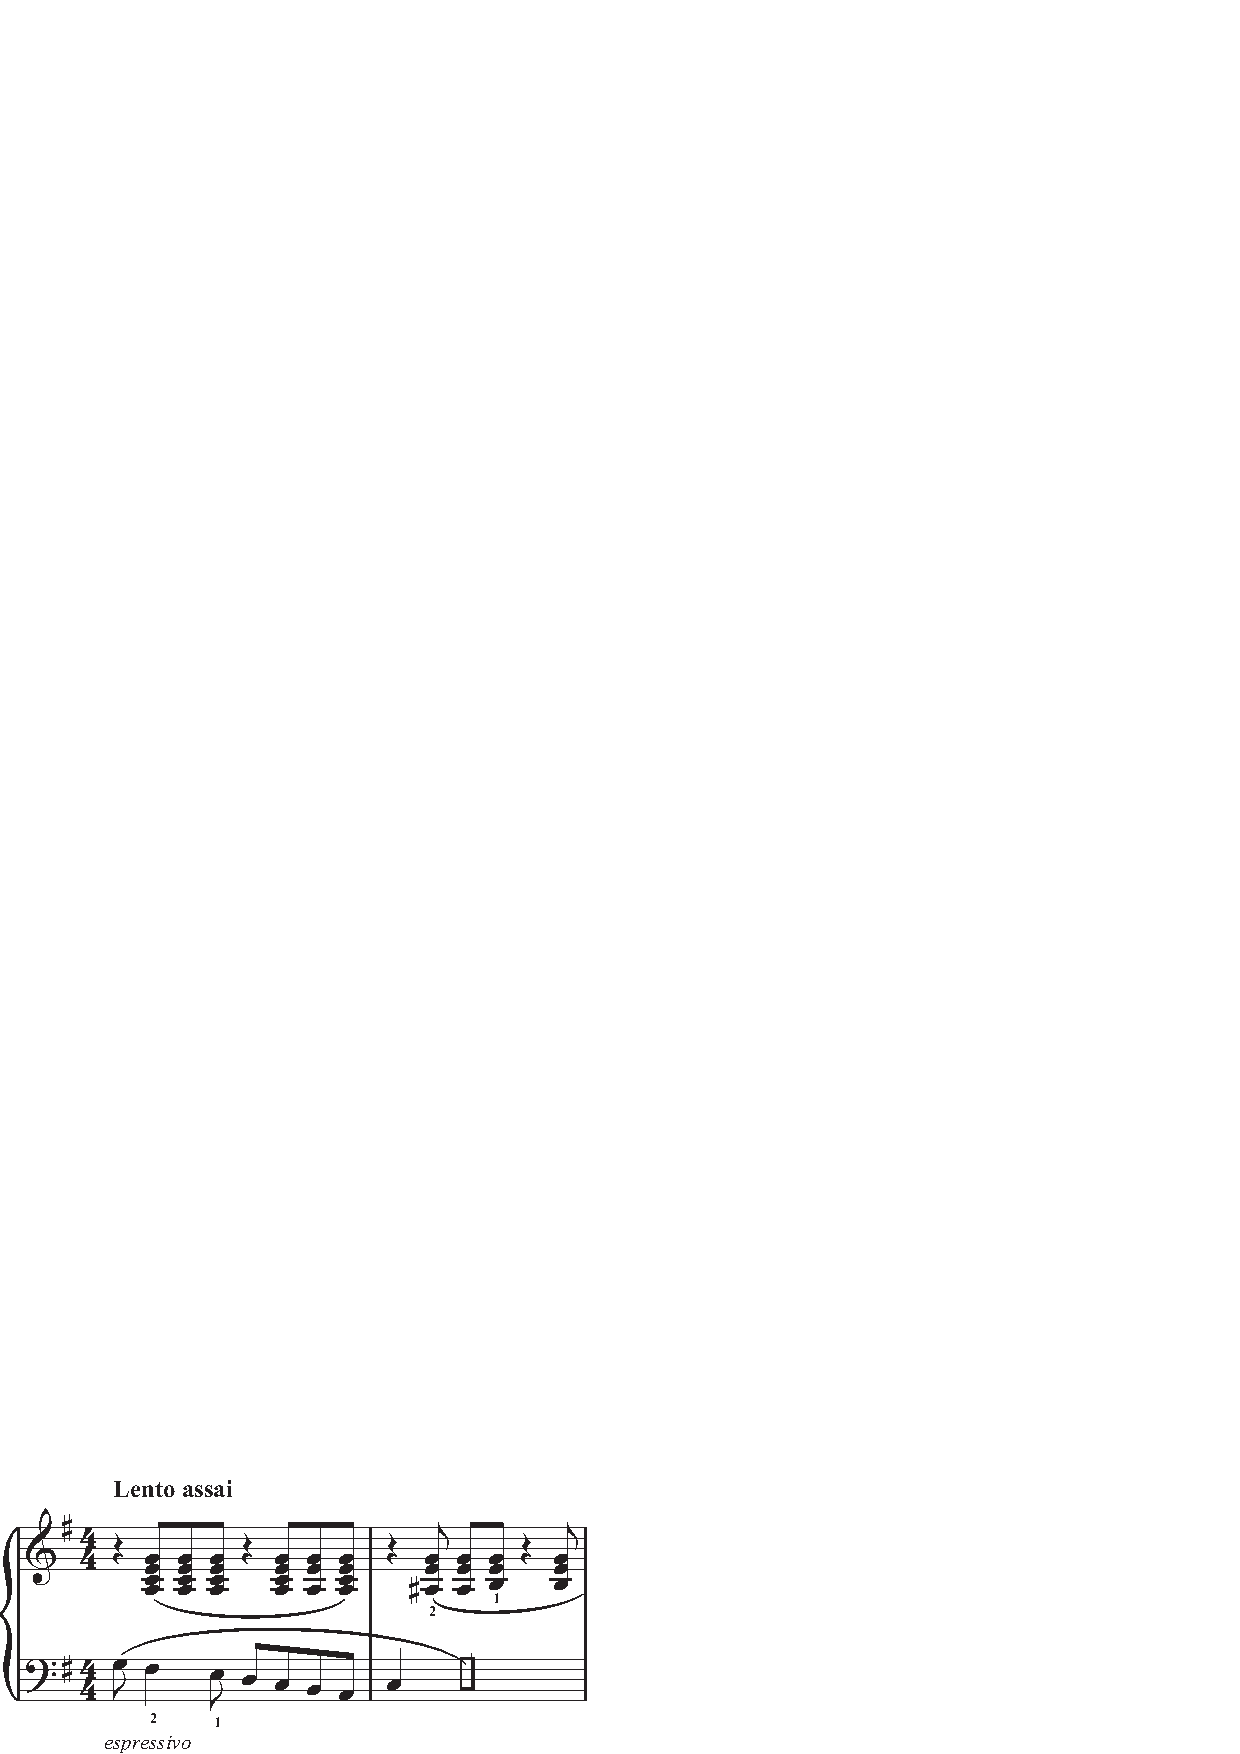
\includegraphics[height=5cm]{obermann.jpg}

\begin{center}
\begin{lilypond}
\version "2.13.34"

\score{
  \new PianoStaff {
    <<
      \new Staff {
        \tempo "Lento assai"
        \key e \minor
        \relative {
        r8 <a c e g>_( q q r8 <a c e g> q q)
        r8 <ais e' g>_( q <b e g> r <b e g> q q) \bar " "
      }}
      \new Staff {
        \clef "bass"
        \relative {
        g8(_\markup{\italic espressivo} fis4 e8 d c b a 
        c4 b2) b4( s4*0)
        }
      }
    >> 
  }
}

\paper{
  oddFooterMarkup = \markup {
    \fill-line {
    } 
  }
}
\end{lilypond}
\end{center}

Les trois notes syncopées de la première mesure établissent d'une part une connexion entre les différentes
fonctions, caractères du thème et d'autre part, il se révèle être le motif porteur des parties de transition et de
développement; il s'agit donc d'un préliminaire au développement cyclique qui arrivera avec la \emph{Sonate en si mineur}.

\subsection{Le thème pastoral}

On rejoint ici l'aspiration d'Obermann à une paix intérieure; mais il sera surtout intéressant de noter que ce
passage décrit la vallée, plus que les états d'âme d'Obermann. On retrouve le motif syncopé, soutenu par 
des accords en croches. 

\begin{center}
\begin{lilypond}
\version "2.13.34"

\score{
  \new PianoStaff {
    <<
      \new Staff {
        \key c \major
        \relative {
        \once \override Staff.TimeSignature #'stencil = ##f

        <<
        {e''4( d2 c4) c( b2 a4)
        a2( fis4. g8 d'4 aes2 g4)
        }
        \\
        {e8 e e e e e e e c c c c c c c c
        c c c c b b b b d d d d d d d d         
        }
        >>
        
      }}
      \new Staff {
        \relative {
         \once \override Staff.TimeSignature #'stencil = ##f

        <c' g'>8 q q q q q q q <a e'> q q q q q q q
        <fis es'>8 q q q <g d'> q q q <ais f'!>8 <ais f'> q q q q q q 
        }
      }
    >> 
  }
}

\paper{
  oddFooterMarkup = \markup {
    \fill-line {
    } 
  }
}
\end{lilypond}
\end{center}

On remarquera aussi, à partir de la mesure 85, les mouvements de basse qui marquent
la progression harmonique.


\subsection{Le thème de la lutte}

On retrouve ici la vision du héros romantique tourmenté, ainsi que tout l'arsenal des moyens mis en \oe{}uvre par Liszt dans
ce type de passage: trémolos, déferlements d'octaves, déplacements rapides; une fois de plus, Liszt fait appel aux trois notes syncopées; cependant, à partir de la mesure 133, il n'utilise plus que deux notes de ce motif; ce procédé, ainsi que l'indication \emph{stringendo} (mesure 137) servent de strette avant l'avalanche d'octaves du presto.

Brusquement, mesure 156, le mouvement de trémolos s'arrête; il laisse la place à une progression chromatique qui, après un long silence, réintroduit le motif syncopé, ponctué d'accords dans le registre grave.

\subsection{Le thème panthéiste}

Le thème de la religion est souvent abordé dans le roman d'Etienne de Senancour; Dieu et nature se mêlent.
Pour Obermann, il y a deux aspects dans cette nature:
\begin{enumerate}
\item elle représente tout d'abord l'idéal perdu par l'homme. Obermann (et Senancour, dont il n'est que le reflet),
essaie de rétablir ce contact avec la nature. En cela, le thème panthéiste rejoint le thème pastoral.
\item la nature symbolise la fuite du temps, la mort. Obermann montre l'importance mineure de l'existence humaine mineure
par rapport à la grandeur de cette nature.
\end{enumerate}

Cette dernière partie de l'\oe{}uvre commence tout d'abord par une passage similaire à celui du thème pastoral;
mais ici, le registre est plus grave, le motif syncopé est accompagné des triolets; cet accompagnement est beaucoup
moins présent et centre l'attention sur le motif principal; ce passage semble décrire le premier aspect de la nature vue
par Obermann.

Vient ensuite un passage, plus lyrique, d'arpégés soutenus par un dessin de doubles croches; il prépare
(surtout dans l'ossia) l'arrivée du final brillant où le motif syncopé est accompagné d'accords en triolets de doubles croches;
l'intensité va grandissante, jusqu'à la coda (mesure 208); là, le motif est traité en strette, jusqu'à un arpège en octave.

On retrouve alors le thème de la première mesure de la pièce (et pas seulement les trois notes syncopées).
On pourra tirer un parallèle avec \emph{The Unanswered Question} de Charles Ives\footcite{ives:unansweredquestion}, dans laquelle la question de l'existence est
énoncée au début de l'\oe{}uvre et, après diverses tentatives de réponses, revient à la fin, restant ainsi sans réponse définitive.

Dans la \emph{Vallée d'Obermann}, le principe de variation dirige le déploiement, la transformation d'une idée
thématique complète sous l'inspiration de l'Obermann de Senancour, de ce roman « d'évolution ».

Cette \oe{}uvre n'est donc pas seulement l'une des « nouvelles formes » annoncées dans la préface de l'\emph{Album
d'un voyageur}, elle n'est pas seulement une nouvelle interprétation du principe de la variation --- cette fois
étendue sur la structure dans sa totalité ---, mais elle est aussi la réalisation la plus frappante de l'union du
programme avec la forme de l'\oe{}uvre. Tous les niveaux de l'action musicale, grâce à la variation, deviennent porteurs de sens, et ce à l'aide d'un
seul thème musical.

La \emph{Vallée d'Obermann} s'impose donc comme une \oe{}uvre majeure: par l'utilisation de la variation d'un seul thème
conducteur, elle anticipe la \emph{Sonate en si mineur}; par le choix du sujet, elle annonce le poème symphonique.

%\section{Bibliographie}

%A. CORNETTE, \emph{Liszt en zijne "Années de Pèlerinage"}, (s. d.)

%\emph{Dictionnaire encyclopédique de la musique}, Université d'Oxford sous la direction de D. ARNOLD (Robert Laffont, collection Bouquins, 1988)

%\emph{Guide de la musique de piano et de clavecin}, sous la direction de F.-R. TRANCHEFORT (Fayard, Les Indispensables de la musique, 1987)

\nocite{cornette} \nocite{tranchefort1987} \nocite{oxford1989} \nocite{liszt:pelerinage1,liszt:pelerinage2} 

\clearpage

\section*{Références}
\addcontentsline{toc}{section}{Références}
\addcontentsline{toc}{subsection}{Ouvrages musicaux}
\printbibliography[heading=theorie, keyword=musique, notkeyword=partition]

\addcontentsline{toc}{subsection}{Partitions}
\printbibliography[heading=partitions, keyword=partition]

 
 \tableofcontents
 
\end{document}
 